\documentclass[final]{beamer}
\usepackage[scale=1.24]{beamerposter}
\usepackage{graphicx,booktabs,tabularx,algorithm,amsmath,caption}
\usepackage[noend]{algpseudocode}
\usepackage{helvet,tikz}

\usetikzlibrary{arrows,fit,patterns}


\usetheme{confposter}
\setbeamercolor{block title}{fg=Maroon,bg=white}
\setbeamercolor{block body}{fg=black,bg=white}
\setbeamercolor{block alerted title}{fg=white,bg=Maroon!70}
\setbeamercolor{block alerted body}{fg=black,bg=Maroon!10}

\newlength{\sepwid}
\newlength{\onecolwid}
\newlength{\twocolwid}
\newlength{\threecolwid}
\setlength{\paperwidth}{48in}
\setlength{\paperheight}{48in}
\setlength{\sepwid}{0.024\paperwidth}
\setlength{\onecolwid}{0.22\paperwidth}
\setlength{\twocolwid}{0.464\paperwidth}
\setlength{\threecolwid}{0.708\paperwidth}
\setlength{\topmargin}{-0.5in}
\newcolumntype{Y}{>{\centering\arraybackslash}X}


\title{Fido: A Universal Robot Control System Using\\Reinforcement Learning with Limited Feedback}
\author{\LARGE Joshua Gruenstein \and Michael Truell}
\institute{\mbox{}}

\begin{document}

\addtobeamertemplate{block end}{}{\vspace*{2ex}}
\addtobeamertemplate{block alerted end}{}{\vspace*{2ex}}
\setlength{\belowcaptionskip}{2ex}
\setlength\belowdisplayshortskip{2ex}

\begin{frame}[t]
\begin{columns}[t]

\begin{column}{\sepwid}\end{column}
\begin{column}{\onecolwid}

	\begin{alertblock}{Control System Objectives}
		Fido was created to fulfill the following goals:
		\begin{itemize}
			\item \textbf{Trainability}: Allow both human and autonomous training and retraining rather than programming
			\item \textbf{Universality}: Run on any robot and perform any task, even without prior knowledge of the host
			\item \textbf{Performance}: Require few learning iterations and low latency for quick and efficient training
		\end{itemize}
		To achieve this we developed a novel machine learning algorithm utilizing wire-fitted Q-Learning with a dynamically resized neural network, a confidence-based probabilistic action selection model, and history sampling.  The control system could be trained at a rate \textbf{4 times} the industry standard, allowing practicality over traditional pre-programmed control systems.
	\end{alertblock}

	\begin{block}{System Overview}
		\begin{algorithm}[H]
		\caption*{\textbf{Fido Control System Algorithm}}\label{euclid}
		\small
		\begin{algorithmic}[1]
			\State Initial empty replay memory $M$
			\State Initial neural network with random weights
			\State Uncertainty value $u \gets \infty$

			\While{$true$}
			  \State Observe state $s_t$
			  \State Feed model $s$ and generate continuous function $r(a)$ of action versus reward
			  \State Select action $a_t$ with expected reward $r_t^*$ using a Softmax action selection policy with temperature $T \propto u$ and the generated $r(a)$ function.

			  \State Execute action $a_t$ and observe reward $r_t$ and new state $s_{t+1}$

			  \State Store ($s_t$, $a_t$, $r_t$, $s_{t+1}$) in $M$

			  \State $u \propto (r_t-r_t^*)^2$

			  \State Sample $n \propto {1/u}$ experiences $e$ giving weight to newer experiences.
			  \State Perform SPSA search on model architectures with cost function as error in predicting $e$ when trained on $e$ using SGD and Adadelta
			  \State Update current model with result of SPSA search
			\EndWhile
		\end{algorithmic}
		\end{algorithm}

		From a macro perspective, Fido can be viewed as a ``black box'' system, where a set of inputs (such as sensors) go in and a set of outputs (actions) go out.  Fido's goal is to maximize given reward by altering its behavior.  The system operates through the following steps:

		\begin{enumerate}
			\item Sensor values are fed to a neural network.
			\item The neural network outputs data points, each is an action and its expected reward.
			\item A wire-fitted least squares interpolator creates a continuous function of action to expected reward using these data points.
			\item An action is chosen using an Softmax selection policy that dynamically adjusts Fido's exploration level as its confidence level changes.
			\item After receiving reward, the neural network is trained to output a new set of data points using Adadelta for gradient descent. Dynamic sizing of the neural network and history sampling are employed to improve neural network performance.
		\end{enumerate}
	\end{block}

\end{column}

\begin{column}{\sepwid}\end{column}

\begin{column}{\twocolwid}

\vspace{-1.65cm}

\begin{columns}[t,totalwidth=\twocolwid]

	\begin{column}{\onecolwid}
		\begin{block}{Reinforcement Learning}
			\begin{itemize}
				\item Fido is a \textbf{reinforcement learning system}. Its goal is to accurately estimate the reward for any action it can perform.
				\item The system uses \textbf{Q-Learning}, a popular reinforcement learning algorithm that develops a function, the ``Q-function'', that intakes a state-action pair and outputs expected utility.
				\item Fido utilizes a \textbf{neural network} coupled with a \textbf{wire-fitted moving least squares interpolator} instead of the traditional table to estimate its Q-function such that relations can be made between similar actions and similar states. Our neural network accepts the state and outputs a few actions along with their expected rewards. Fido interpolates these action-reward pairs to create a continuous function of action to reward.
				\item Once Fido performs an action and receives a reward (a single \textbf{reward iteration}), the control system calculates its \textbf{uncertainty value} as the difference between its expected reward and the real reward that it has received. Higher uncertainty means that Fido is still learning or is undergoing retraining.
				\item Fido selects actions to perform using a probabilistic Softmax policy which gives greater weight to actions with greater expected utility, but allows for exploration.
				\begin{itemize}
					\item Fido dynamically adjusts its exploration level to be proportional to its uncertainty value.
					\item This allows Fido to continuously execute the best actions possible once it has been trained and is sure of its actions, but also allows it to explore when being retrained.  This allows for lower training times and higher average reward.
				\end{itemize}
			\end{itemize}
		\end{block}
	\end{column}

	\begin{column}{\onecolwid}\begin{block}{Training}

	\begin{figure}
		\centering
		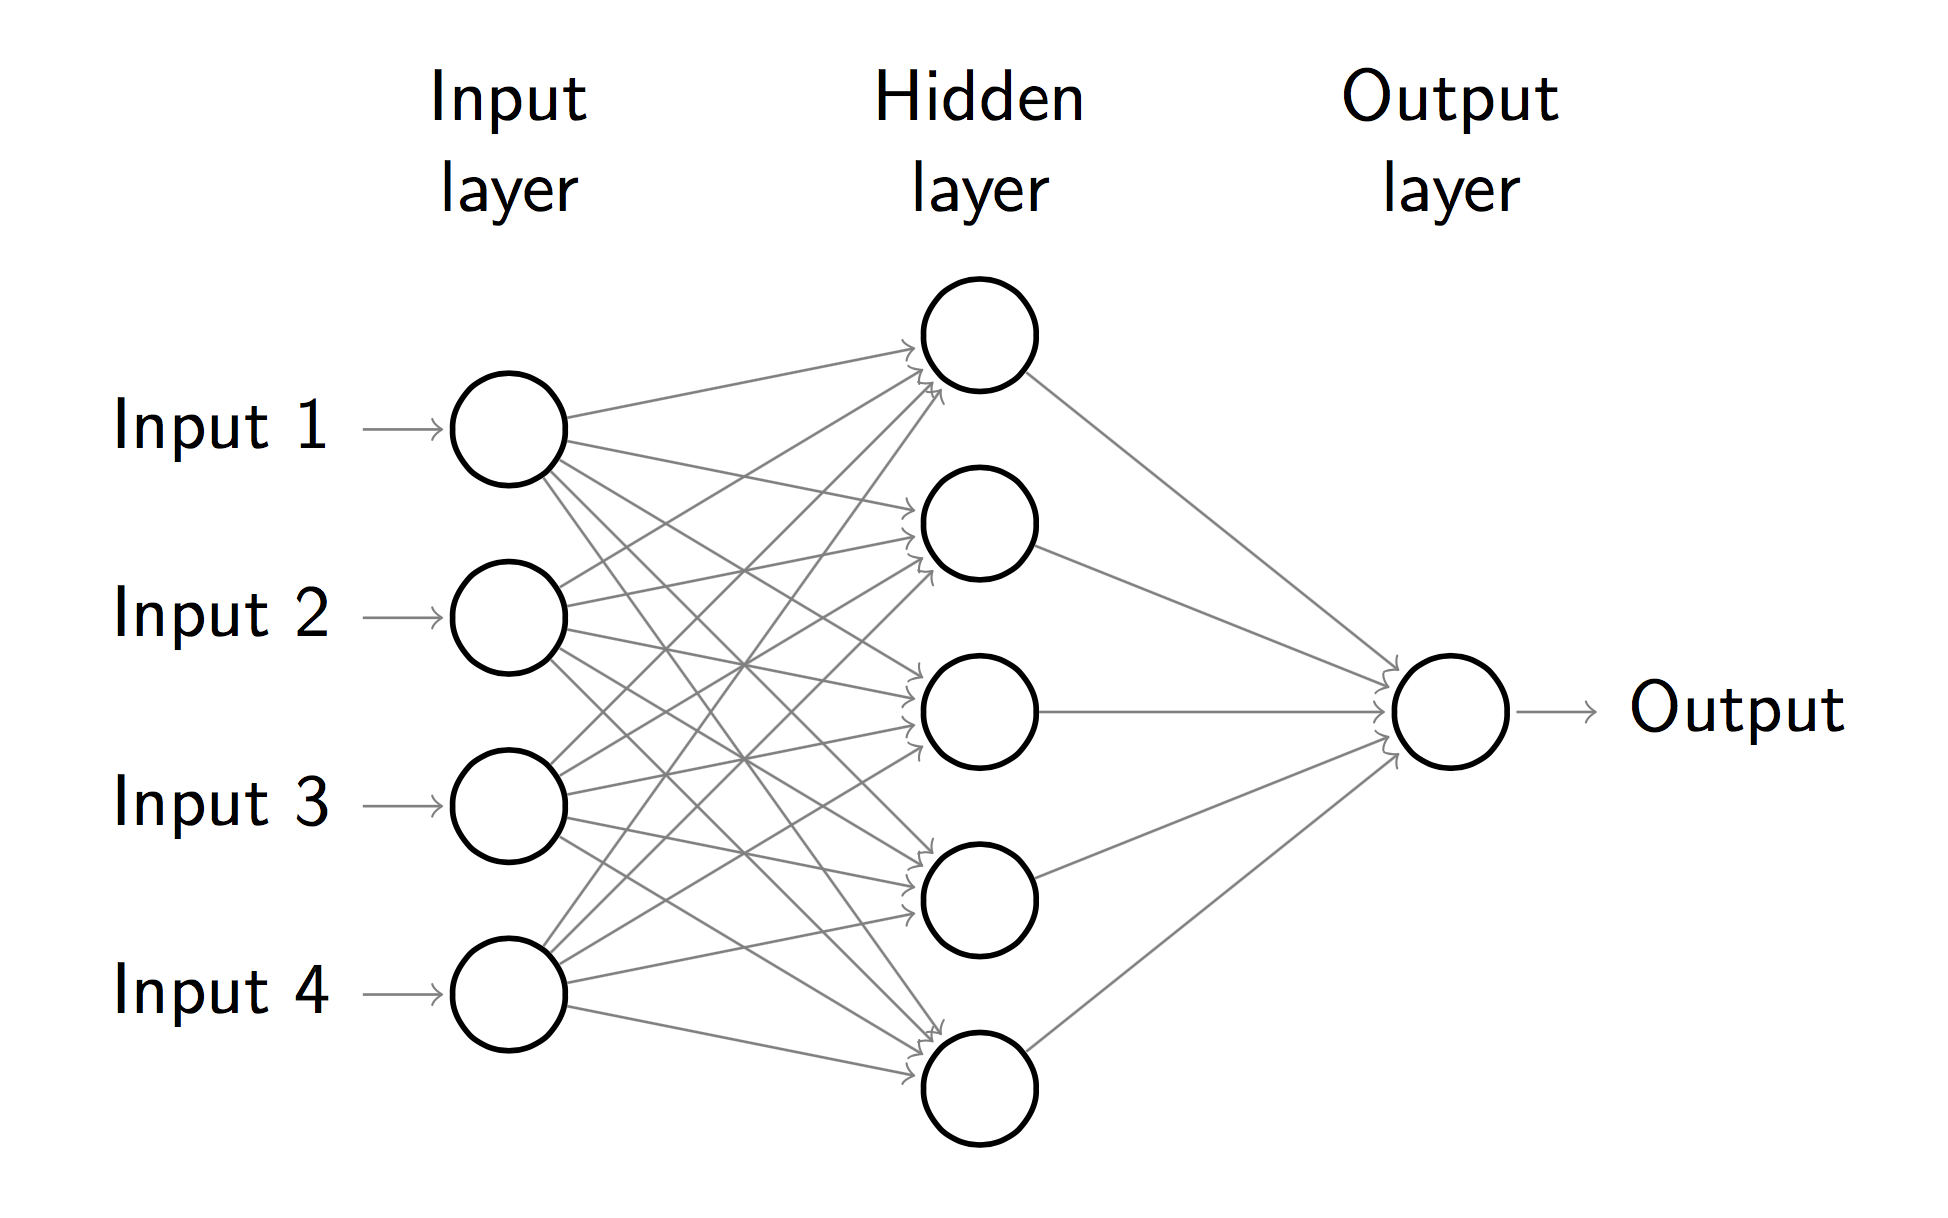
\includegraphics[width=.8\linewidth]{Figures/FeedForwardRendered}
		\caption{Single Output Feed-forward Neural Network}
		\label{fig:feedforward}
	\end{figure}

	\begin{itemize}
		\item After every reward iteration, Fido adjusts its model to correct the disparity between its expected reward and the reward it just recieved using \textbf{Stochastic Gradient Descent} to modify the action-reward pairs that are outputted by its neural network.
		\item Fido trains its neural network using the Adadelta training method, eliminating the need to specify a hard-coded learning rate.
		\item Fido uses \textbf{experience replay}, the practice of training a system on past states, actions, and rewards to decrease training time. Fido gives weight to newer experiences. If uncertainty value of the model begins to rise, Fido samples fewer experiences, because past rewards will be incorrect if Fido is being trained on a new task.
		\item After each reward iteration, Fido efficiently grows and prunes its neural network to the optimal size and architecture for the task at hand, using neuron sensitivity approximations.
	\end{itemize}

\end{block}

\end{column}

\end{columns}
	\vspace{-1cm}
	\begin{block}{Results}
		Results were gathered both from simulation and hardware for a variety of tasks.    Gathered data for each task included the number of learning iterations, or how many pieces of reward it took for Fido to master the task, action selection time, and training time, or latency in updating Fido's model.
		\begin{table}[ht]
			\centering
			\caption {Fido Results in Simulation (400 trials per task)} \label{tab:simresults}
			\vspace{-1cm}
			\begin{tabularx}{.9\textwidth}{l||Y|Y|Y}
				\toprule
				Task        & Learning Iterations & Action Selection (ms) & Training Time (ms) \\ \midrule
				Flash       & 3                  & 0.                    & 6                  \\
				Float to Point       & 14         & 1                     & 6                  \\
				Drive to Point       & 16         & 1                     & 11                 \\
				Line Following       & 10         & 0.                    & 2                  \\
				Noisy Line Following & 13         & 0.                    & 105                \\
				\bottomrule
			\end{tabularx}
		\end{table}
		\vspace{.5cm}

		\begin{table}[ht]
			\centering
			\caption {Fido Results on Thing One (20 trials per task)} \label{tab:thingoneresults}
			\vspace{-1cm}
			\begin{tabularx}{.9\textwidth}{l||Y|Y|Y}
				\toprule
				Task              & Learning Iterations & Action Selection (ms) & Training Time (ms) \\ \midrule
				Stay Still        & 3                   & 1                    & 43.5                  \\
				Drive to Point    & 18                  & 4                     & 65                  \\
				\bottomrule
			\end{tabularx}
		\end{table}

		\begin{table}[ht]
			\centering
			\caption {Fido Results on Thing Two (20 trials per task)} \label{tab:thingtworesults}
			\vspace{-1cm}
			\begin{tabularx}{.9\textwidth}{l||Y|Y|Y}
				\toprule
				Task              & Learning Iterations & Action Selection (ms) & Training Time (ms) \\ \midrule
				Drive Straight         & 13                   & 2                    & 30                 \\
				Line Following         & 15                  & 21                    & 95                \\
				Fetch                  & 8                  & 1                     & 70                 \\
				Limping Line Following & 6                   & 20                    & 37                 \\
				\bottomrule
			\end{tabularx}
		\end{table}

		\begin{table}[ht]
			\centering
			\caption {Fido Results on Thing Three (20 trials per task)} \label{tab:thingtworesults}
			\vspace{-1cm}
			\begin{tabularx}{.9\textwidth}{l||Y|Y|Y}
				\toprule
				Task              & Learning Iterations & Action Selection (ms) & Training Time (ms) \\ \midrule
				Draw Square         & 5                   & 5                    & 4                 \\
				Ping Pong          & 12                  & 3                    & 128                \\
				\bottomrule
			\end{tabularx}
		\end{table}

	\end{block}

\end{column}

\begin{column}{\sepwid}\end{column}

\begin{column}{\onecolwid}
	\begin{block}{Fido vs. Discrete Q-Learning}
		Fido's performance in completing various simulator tasks was tested against the industry standard of discrete Q-Learning using a neural network.  On average Fido required \textbf{four times fewer} learning iterations than discrete Q-Learning for a given task.
		\vspace{0.1cm}
		\begin{table}[ht]
			\centering
			\caption {Fido Results Compared to Discrete Q-Learning} \label{tab:simresults}
			\vspace{-1cm}
			\small
			\begin{tabularx}{.9\textwidth}{lYY}
				\toprule
				Task        & Fido Learning Iterations & Discrete Learning Iterations \\ \midrule
				Flash             & 3   & 16  \\
				Float to Point    & 14  & 56  \\
				Drive to Point    & 16  & 69  \\
				Line Following    & 10  & ??? \\
				\bottomrule
			\end{tabularx}
		\end{table}
	\end{block}
	\begin{block}{Implementation}
		\setlength\parindent{48pt}
		\indent The Fido control system was programmed in C++, with no external dependencies. Three hardware implementations and a simulator were constructed to test Fido's performance.  The first robot utilized a differential drive system and was powered by an Intel Edison, the second used a holonomic 3x swedish 90 degree wheel arrangment and ran on a \$5 Raspberry Pi Zero, while the third was a 4-axis jointed arm running of a Raspberry Pi Zero.

		\begin{figure}
			\centering
			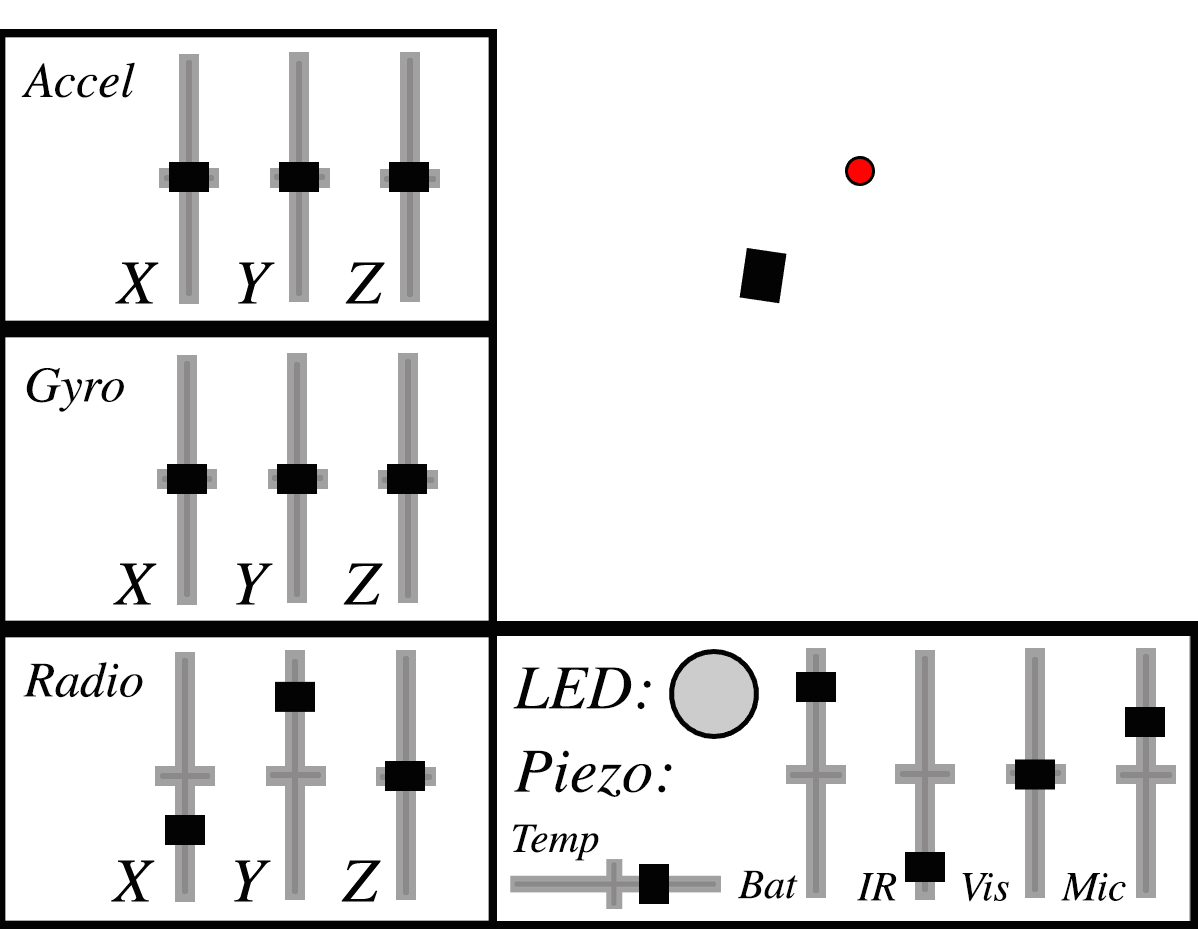
\includegraphics[width=.6\linewidth]{Figures/Screenshot.png}
			\caption{Fido Simulator Graphical User Interface}
		\end{figure}

		\vspace{-0.5in}

		\begin{figure}[ht]
			\centering
			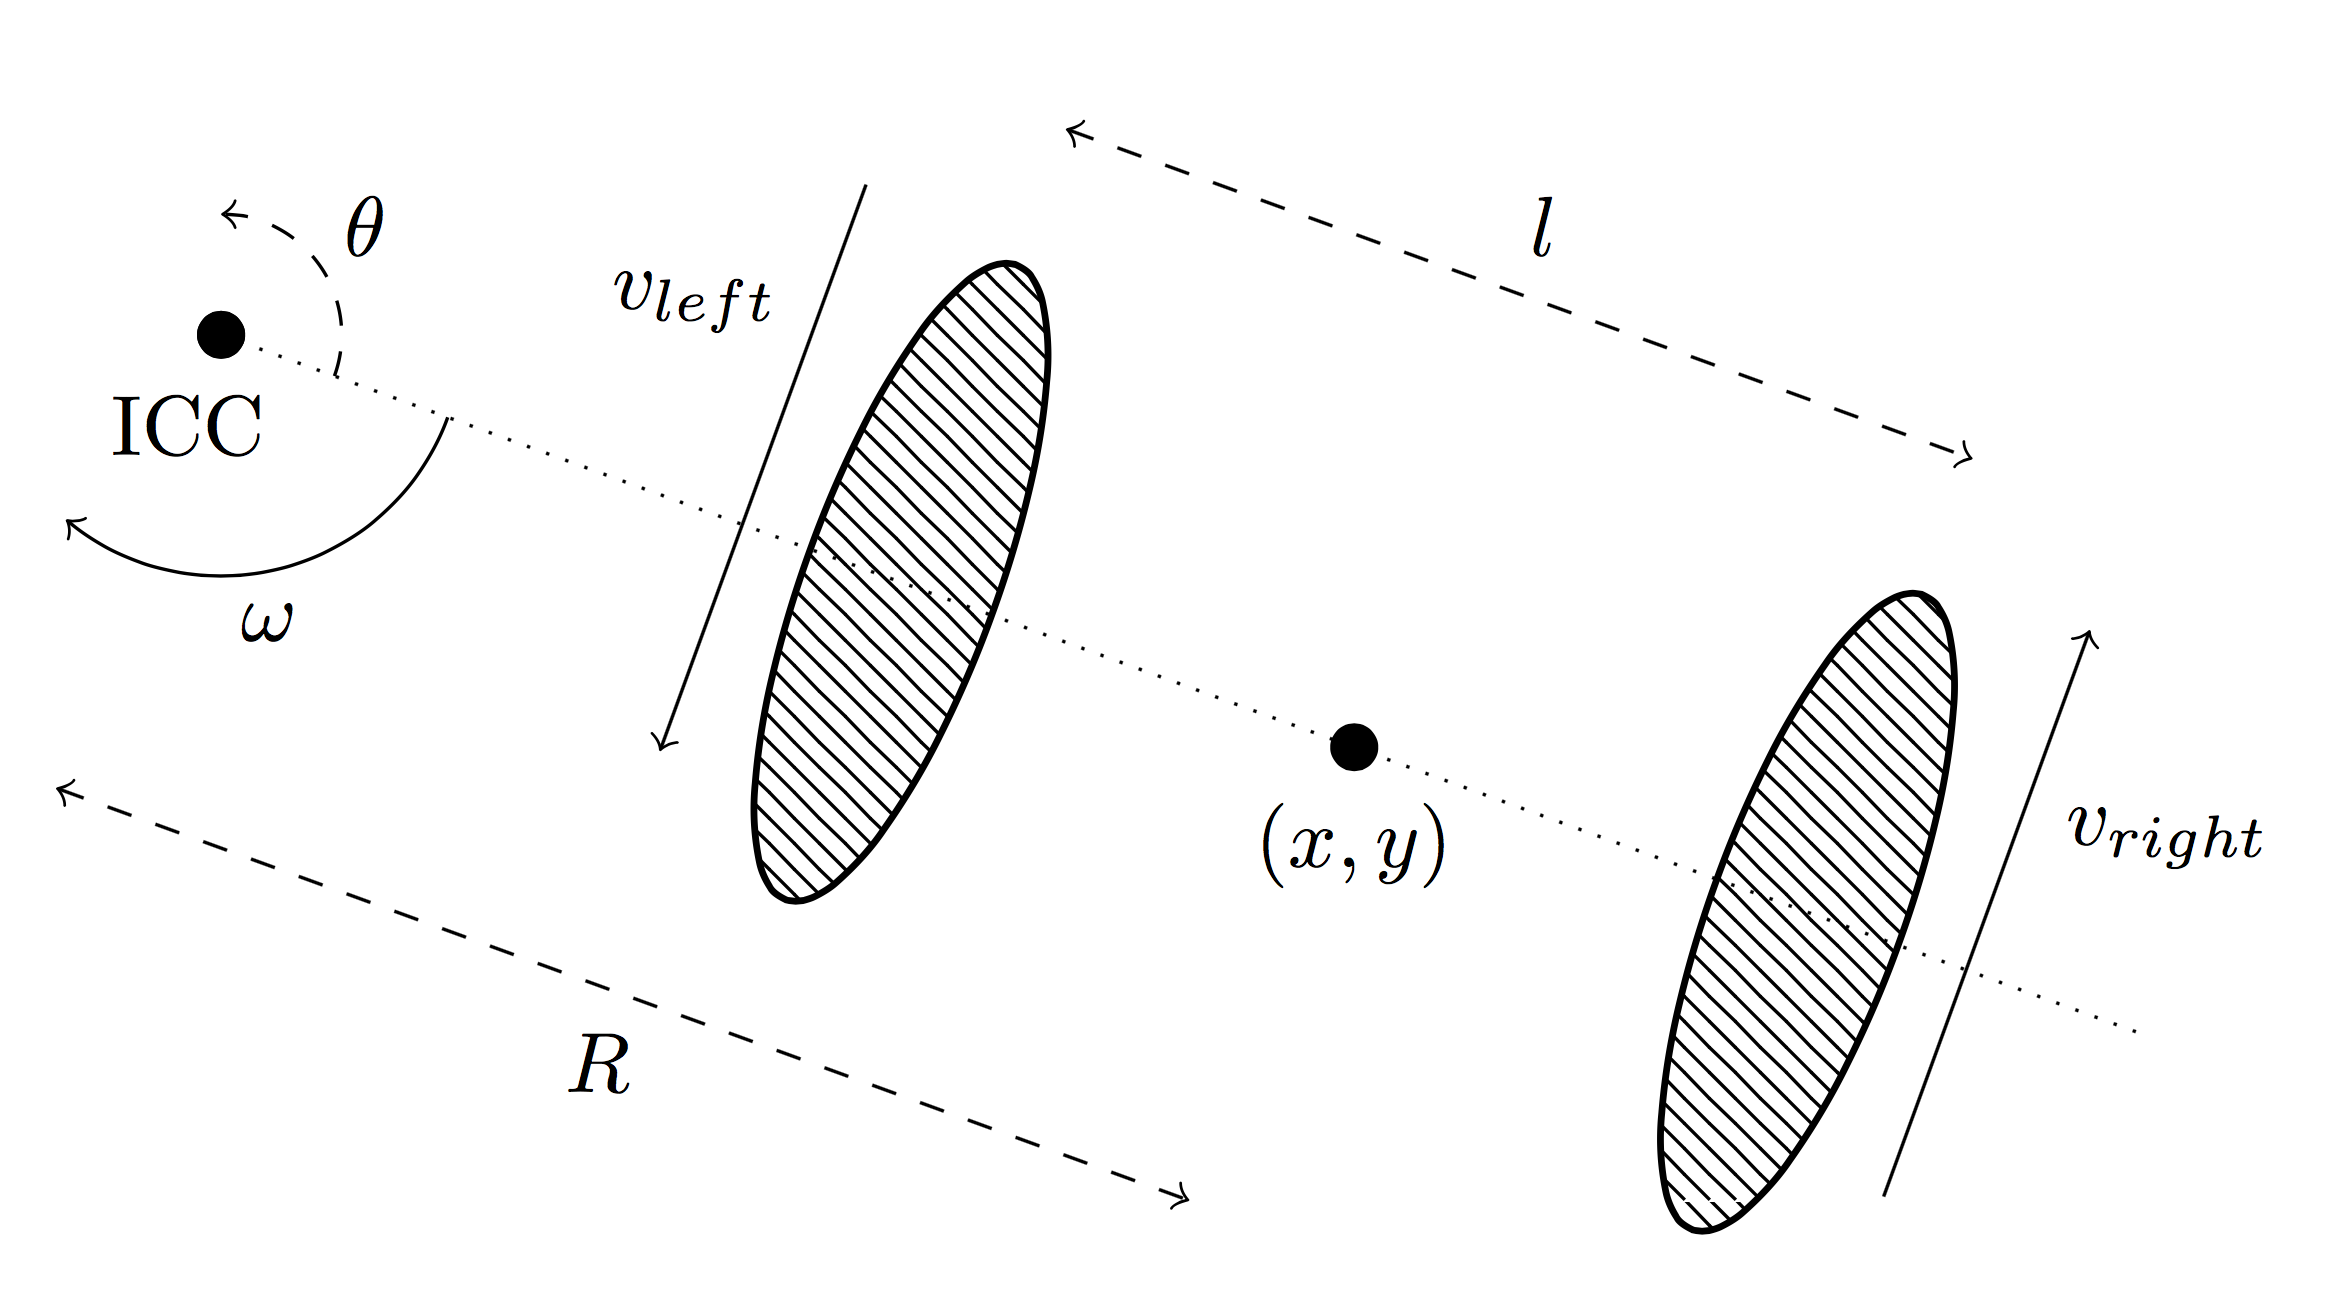
\includegraphics[height=.4\linewidth]{Figures/differentialKinematicsRendered.png}
			\caption{Differential Drive Kinematics}
		\end{figure}

		\vspace{-0.5in}

		\begin{figure}[ht]
			\centering
			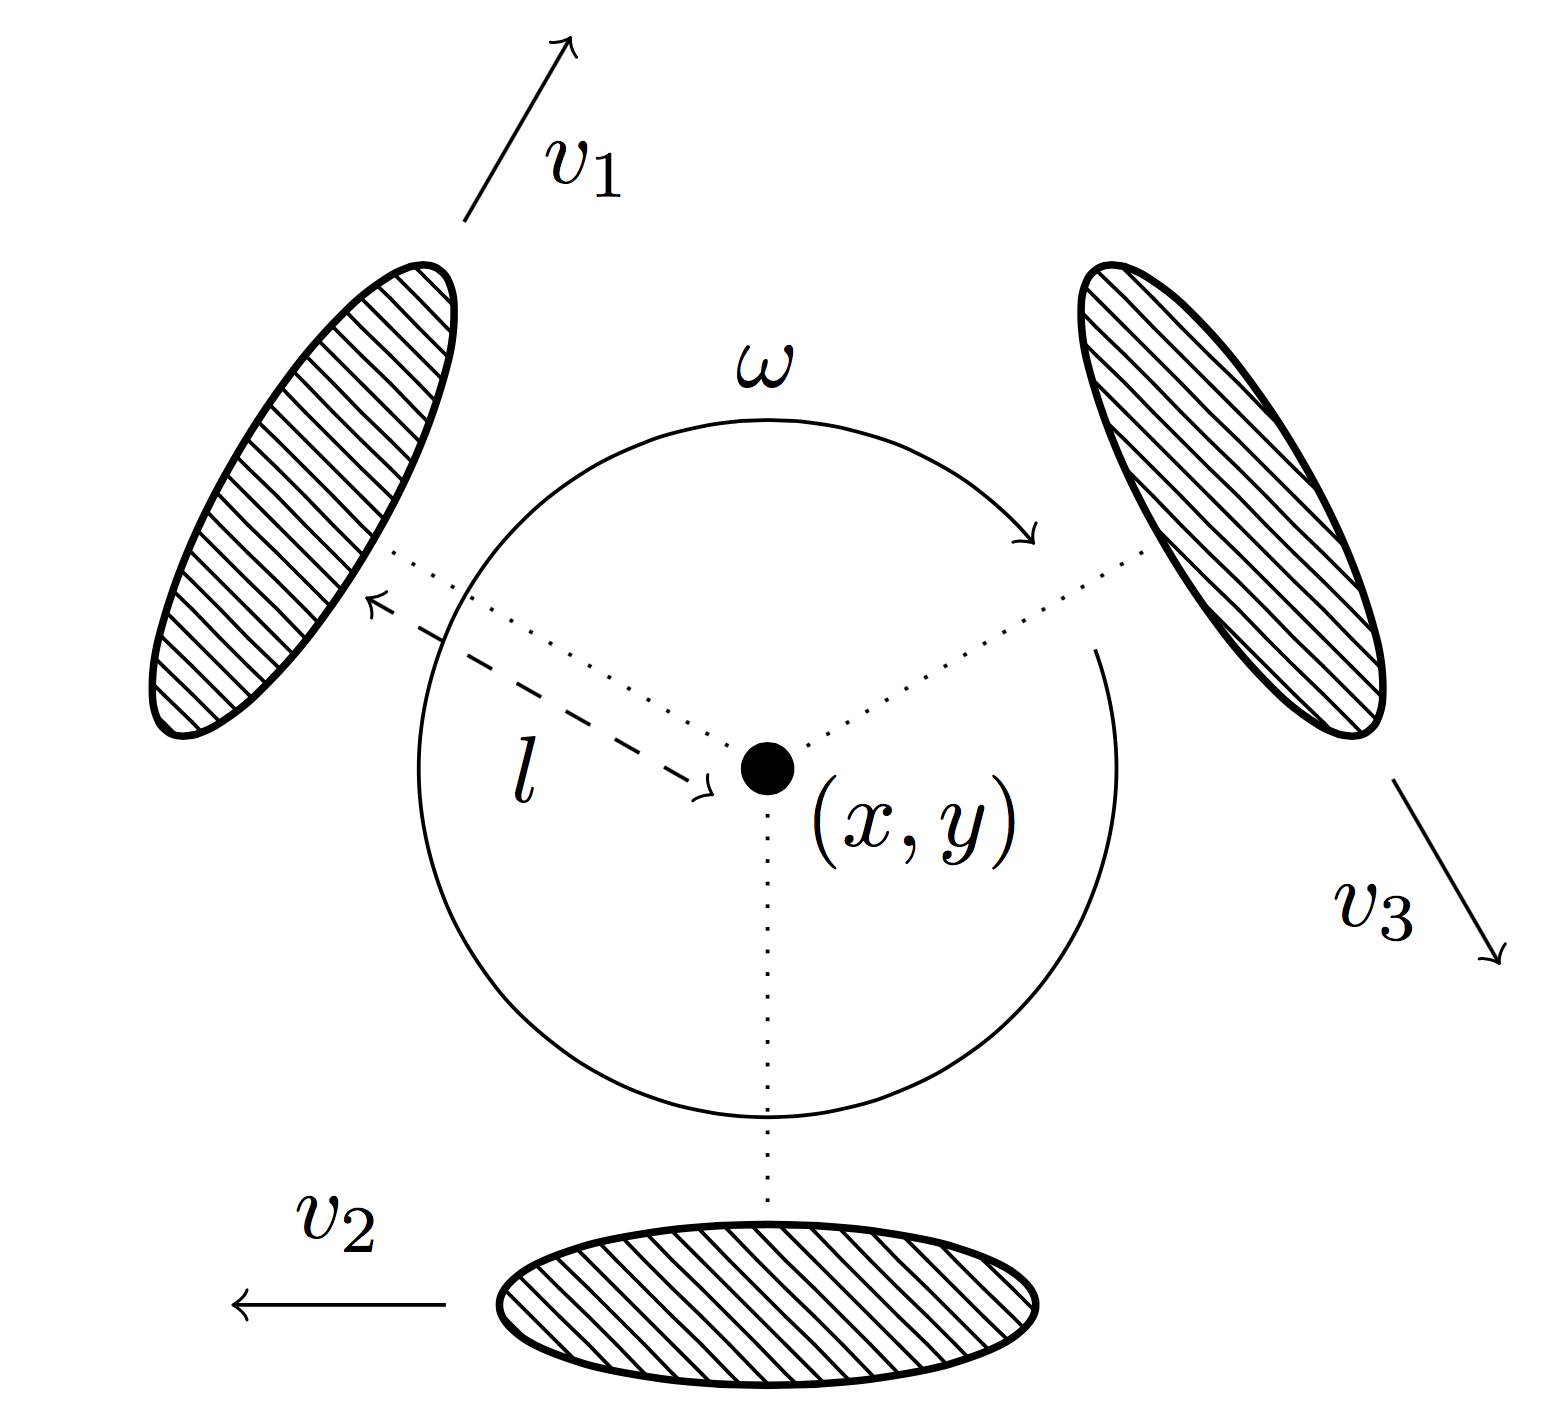
\includegraphics[height=.4\linewidth]{Figures/kiwiKinematicsRendered.png}
			\caption{Holonomic Kiwi Drive Kinematics}
		\end{figure}
	\end{block}

	\begin{block}{Applications}
		Fido provides numerous advantages over traditional procedural-programmed control systems, making it practical for a number of real world applications.  As Fido can be trained and retrained without expert knowledge, it could be useful in making robotics more accessible to consumers and small-buisness owners.  Fido can also be retrained to adapt to new and unexpected circumstances such as malfunctions in the field, an advantageous feature for militiary applications.
	\end{block}

	\begin{block}{Selected References}
		\nocite{*}
		{\fontsize{25}{30}\bibliographystyle{IEEEtran}\bibliography{Poster}\vspace{0.75in}}
	\end{block}

\end{column}

\end{columns}
\end{frame}
\end{document}

%%%%%%%%%%%%%%%%%%%%%%%%%%%%%%%%%%%%%%%%%
% Adapted from "Jacobs Landscape Poster"
% https://teamwork.jacobs-university.de:8443/confluence/display/CoPandBiG/LaTeX+Poster
% License: CC BY-NC-SA 3.0 (http://creativecommons.org/licenses/by-nc-sa/3.0/)
%%%%%%%%%%%%%%%%%%%%%%%%%%%%%%%%%%%%%%%%%
